\documentclass[12pt]{article}
\usepackage{amsmath, amssymb, amsthm, amsfonts, geometry}
\usepackage{graphicx}
\newtheorem{theorem}{Theorem}
\newtheorem{lemma}{Lemma}
\newtheorem{proposition}{Proposition}
\newtheorem{corollary}{Corollary}
\newtheorem{definition}{Definition}

% Page Setup
\geometry{top=1in, bottom=1in, left=1in, right=1in}

\title{Dat102 Oblig 3}
\author{Thobias K. Høivik} %,Gunnar Salbu, Birk Tangen, Glenn Boine}
\date{\today}

\begin{document}

\maketitle
\section*{Uke 10 d) Tidskompleksitetsanalyse}

Vi skal analysere tidskompleksiteten for følgende metoder for \texttt{TabellMengde} (array-basert mengde) og \texttt{LenketMengde} (lenket liste-basert mengde). Vi bruker \textit{O-notasjon} for å uttrykke kjøretiden, og tar med både beste og verste tilfelle der det er forskjell.

\subsection*{i. \texttt{boolean inneholder(T element)}} - \textit{Sjekk om et element finnes i mengden}

\textbf{TabellMengde} (Array-basert mengde):
\begin{itemize}
    \item \textbf{Beste tilfelle}: Elementet finnes i første posisjon, som tar konstant tid, \(O(1)\).
    \item \textbf{Verste tilfelle}: Elementet er på siste posisjon eller ikke i mengden i det hele tatt, og vi må iterere gjennom hele arrayet, som tar lineær tid, \(O(n)\).
\end{itemize}

Så, for \texttt{TabellMengde}, er tidskompleksiteten:
\[
\text{Beste tilfelle}: O(1), \quad \text{Verste tilfelle}: O(n)
\]

\textbf{LenketMengde} (Lenket liste-basert mengde):
\begin{itemize}
    \item \textbf{Beste tilfelle}: Elementet er i hodet av listen, og tar konstant tid, \(O(1)\).
    \item \textbf{Verste tilfelle}: Elementet er på slutten av listen eller ikke i listen, og vi må traversere hele listen, som tar lineær tid, \(O(n)\).
\end{itemize}

Så, for \texttt{LenketMengde}, er tidskompleksiteten:
\[
\text{Beste tilfelle}: O(1), \quad \text{Verste tilfelle}: O(n)
\]

\subsection*{ii. \texttt{boolean erDelmengdeAv(MengdeADT<T> annenMengde)}} - \textit{Sjekk om mengden er en delmengde av en annen mengde}

\textbf{TabellMengde} (Array-basert mengde):
\begin{itemize}
    \item \textbf{Beste tilfelle}: Hvis første element ikke finnes i den andre mengden, kan vi umiddelbart returnere \texttt{false}, som tar \(O(1)\).
    \item \textbf{Verste tilfelle}: Vi må sjekke hvert element i den nåværende mengden for å se om det finnes i den andre mengden. For hvert element i den nåværende mengden, sjekker vi om det finnes i den andre mengden, som tar \(O(n)\) for hvert av de \(n\) elementene, som gir en total tidskompleksitet på \(O(n^2)\).
\end{itemize}

Så, for \texttt{TabellMengde}, er tidskompleksiteten:
\[
\text{Beste tilfelle}: O(1), \quad \text{Verste tilfelle}: O(n^2)
\]

\textbf{LenketMengde} (Lenket liste-basert mengde):
\begin{itemize}
    \item \textbf{Beste tilfelle}: Hvis første element ikke finnes i den andre mengden, kan vi umiddelbart returnere \texttt{false}, som tar \(O(1)\).
    \item \textbf{Verste tilfelle}: Vi må sjekke hvert element i den nåværende mengden, som innebærer å sjekke om hvert element er i den andre mengden. Dette krever å traversere begge listene, og derfor tar det \(O(n^2)\) i verste tilfelle, der \(n\) er antall elementer.
\end{itemize}

Så, for \texttt{LenketMengde}, er tidskompleksiteten:
\[
\text{Beste tilfelle}: O(1), \quad \text{Verste tilfelle}: O(n^2)
\]

\subsection*{iii. \texttt{boolean erLik(MengdeADT<T> annenMengde)}} - \textit{Sjekk om mengden er lik en annen mengde}

\noindent
\textbf{TabellMengde} (Array-basert mengde):

\noindent 
For å se om to mengder er like, matematisk, innebærer å sjekke om de to mengdene 
        er delmengder av hverandre. Så hvis de har forskjellig kardinalitet 
        vil de ikke være like. Desverre ville dette involvert å se gjennom begge 
        mengdene før vi gjør noe mer så vår metode kaller bare hver mengde sin 
        er \texttt{delMengdeAv()} metode siden vi ikke kan spare noe meningsful tid.  
\begin{itemize}
    \item \textbf{Beste tilfelle:} \texttt{erDelMengdeAv} \(\rightarrow O(1)\). 
        Vi kaller metoden to ganger som gir oss, men dette simplifiseres til \(O(1)\). 
    \item textbf{Verste tilfelle:} Igjen for vi det dobbelte av \texttt{erDelMengdeAv},
        men \(2n^2\) simplifiseres til \(n^2\) så vi sitter igjen med \(O(n^2)\).

\end{itemize}

Så, for \texttt{TabellMengde}, er tidskompleksiteten:
\[
\text{Beste tilfelle}: O(1), \quad \text{Verste tilfelle}: O(n^2)
\]

\noindent 
\textbf{LenketMengde} (Lenket liste-basert mengde):

\noindent 
For akkurat samme grunner som i TabellMengde seksjonen får vi

\noindent 
\texttt{LenketMengde}:
\[
\text{Beste tilfelle}: O(1), \quad \text{Verste tilfelle}: O(n^2)
\]

\subsection*{iv. \texttt{MengdeADT<T> union(MengdeADT<T> annenMengde)}} - \textit{Union av to mengder}

\textbf{TabellMengde} (Array-basert mengde):
\begin{itemize}
    \item \textbf{Beste tilfelle}: Hvis begge mengdene er tomme, 
        lager vi og returnerer vi bare en mengde som tar \(O(1)\).
    \item \textbf{Verste tilfelle}: Vi må traversere begge mengdene. 
        I verste tilfelle, hvis begge mengdene har \(n\) elementer, 
        tar det \(O(n)\) for å traversere begge mengdene og \(O(n)\) 
        for å kopiere resultatet til en ny array. Så, tidskompleksiteten er \(O(n)\). 
\end{itemize}

Så, for \texttt{TabellMengde}, er tidskompleksiteten:
\[
\text{Beste tilfelle}: O(1), \quad \text{Verste tilfelle}: O(n)
\]

\textbf{LenketMengde} (Lenket liste-basert mengde):
\begin{itemize}
    \item \textbf{Beste tilfelle}: Samme igjen viss begge mengdene er tomme: \(O(1)\).
    \item \textbf{Verste tilfelle}: Vi må traversere begge lenkede listene og sette inn alle elementene fra den andre listen i den første. Dette krever å besøke alle elementene i begge listene, og tar derfor \(O(n)\).
\end{itemize}

Så, for \texttt{LenketMengde}, er tidskompleksiteten:
\[
\text{Beste tilfelle}: O(1), \quad \text{Verste tilfelle}: O(n)
\]

\subsection*{v. \texttt{T fjern(T element)}} - \textit{Fjern et element fra mengden}

\textbf{TabellMengde} (Array-basert mengde):
\begin{itemize}
    \item \textbf{Beste tilfelle}: Elementet er på første posisjon,
        og vi kan bare bytte dette elementet med det siste og fjerne det siste. 
        Dette tar \(O(1)\). Alternativt er mengden tom og det tar fortsatt \(O(1)\)
    \item \textbf{Verste tilfelle}: Elementet er på siste posisjon eller finnes ikke i det hele tatt, og vi må traversere hele arrayet før vi kan fjerne elementet. Dette tar\(O(n)\).
\end{itemize}

Så, for \texttt{TabellMengde}, er tidskompleksiteten:
\[
\text{Beste tilfelle}: O(1), \quad \text{Verste tilfelle}: O(n)
\]

\textbf{LenketMengde} (Lenket liste-basert mengde):
\begin{itemize}
    \item \textbf{Beste tilfelle}: Elementet er i hodet av listen eller hodet finnst ikke,
        og vi kan bare oppdatere pekerne/gjøre ingenting. Dette tar \(O(1)\).
    \item \textbf{Verste tilfelle}: Vi må traversere hele listen for å finne elementet, som tar \(O(n)\).
\end{itemize}

Så, for \texttt{LenketMengde}, er tidskompleksiteten:
\[
\text{Beste tilfelle}: O(1), \quad \text{Verste tilfelle}: O(n)
\]

\section*{Oppsummering av tidskompleksiteter}

\[
\begin{array}{|c|c|c|c|c|}
\hline
\text{Metode} & \text{Tabell Beste} & \text{Tabell Verste} 
              & \text{Lenket Beste} 
              & \text{Lenket Verste} \\
\hline
\text{i. inneholder()} & O(1) & O(n) & O(1) & O(n) \\
\text{ii. erDelmengdeAv() } & O(1) & O(n^2) & O(1) & O(n^2) \\
\text{iii. erLik() } & O(1) & O(n^2) & O(1) & O(n^2) \\
\text{iv. union() } & O(1) & O(n) & O(1) & O(n) \\
\text{v. fjern()} & O(1) & O(n) & O(1) & O(n) \\
\hline
\end{array}
\]

\section*{Uke 10 e) HashSet \& TreeSet vs. Tabell \& Lenket }
Generellt når vi gjorde praktiske hastighetstester mellom Lenket- og Tabellmengde 
vs. HashSet, som vi bruket i JavaSetToMengde implementasjonen, observerte vi 
en hastighetsforskjell på to størrelsesordener; en enorm forskjell. 
Når det gjelder sammenligning mellom Lenket- og Tabellmengde observerte vi i våre tester at 
tabellmengde som oftest var litt raskere. Med HashSet og TreeSet står det på nettet at 
HashSet som oftest har bedre kompleksitet, gjern \(O(1)\) når TreeSet er \(O()\).  
Den store fordelen for TreeSet er vistnok er sortert og kan da traverserest effektivt. 
TreeSet har også noen ekstra metoder som egner seg til noen bruksområder.

\begin{figure}[h]
    \centering
    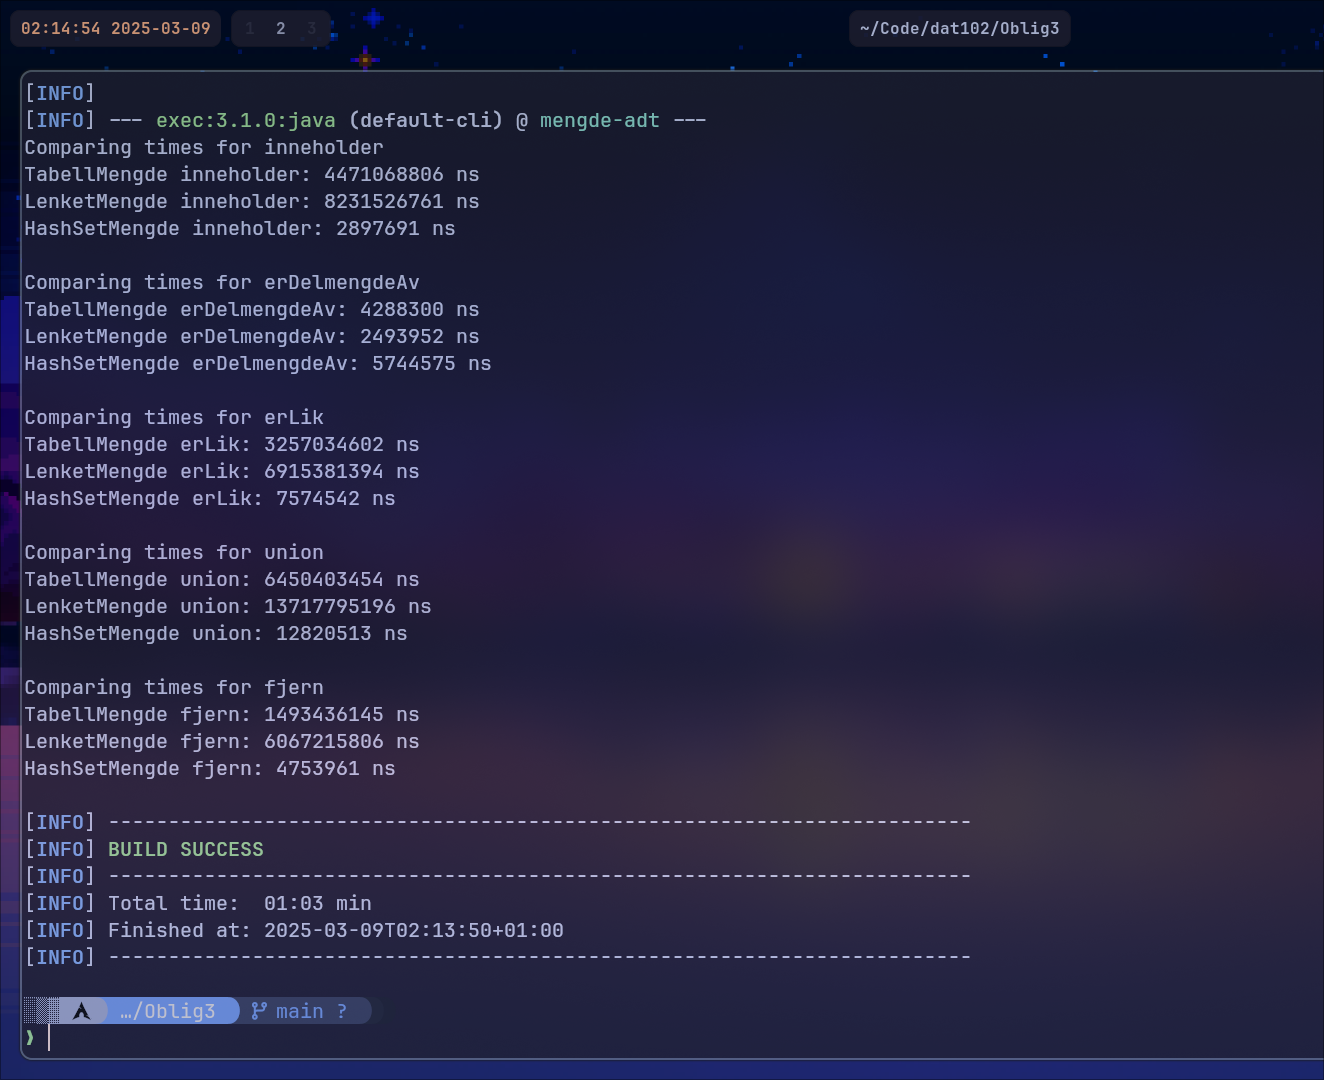
\includegraphics[width=0.8\textwidth]{./EffektivitetsSammenligning.png} 
    \caption{Kjøretider}
    \label{fig:runtimes}
\end{figure}

\section*{Uke 11 f)} 
\begin{figure}[h]
    \centering
    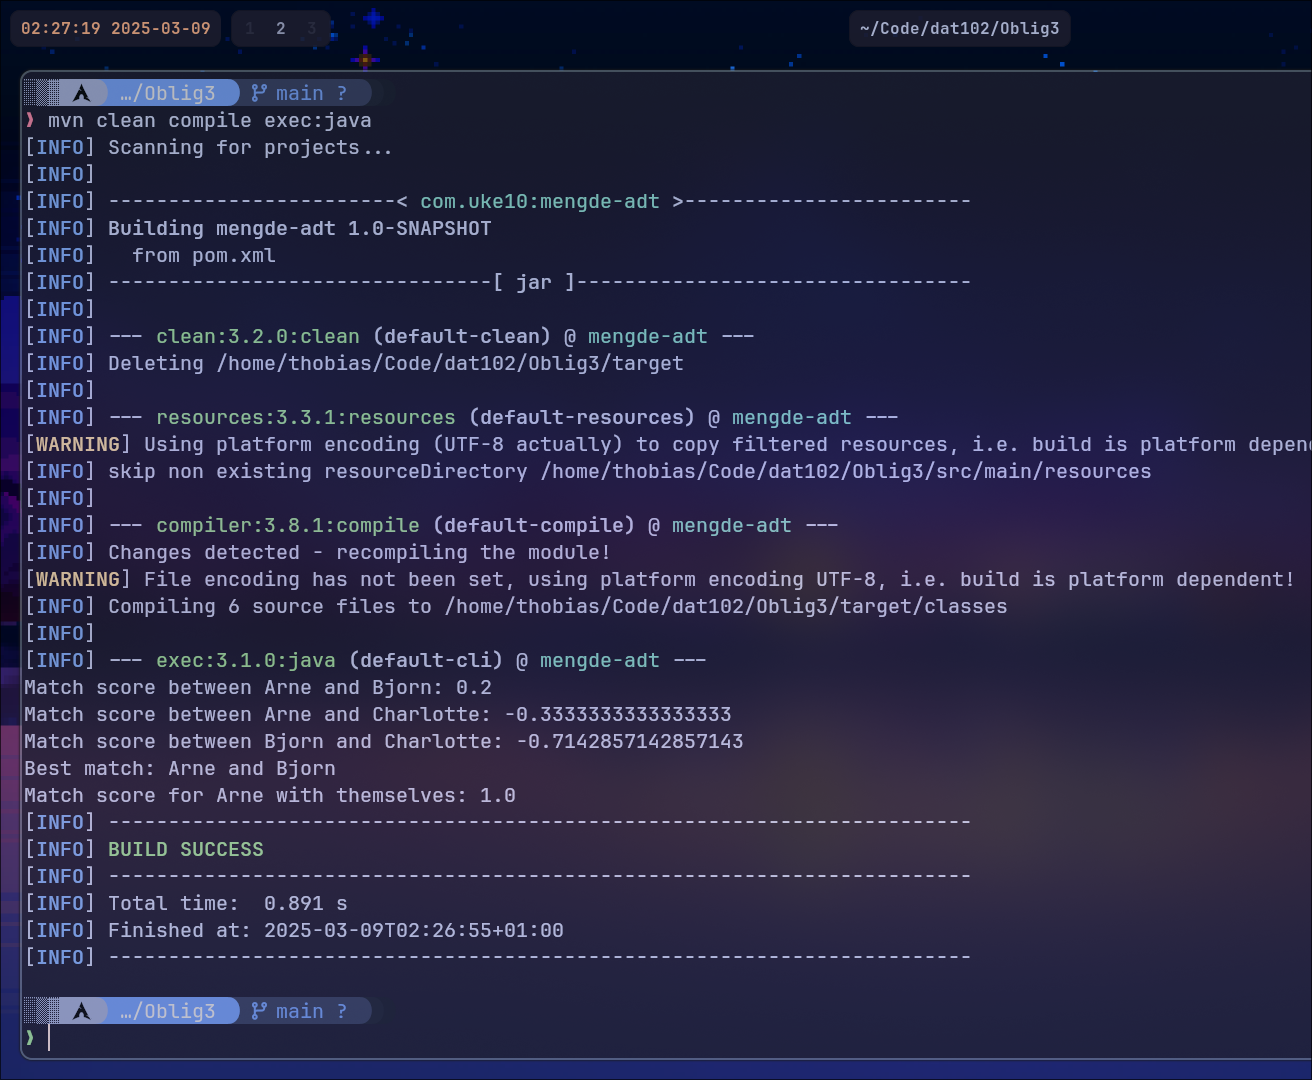
\includegraphics[width=0.8\textwidth]{./Match.png} 
    \caption{Match}
    \label{fig:match}
\end{figure}




\end{document}
